\section{Background}
The target audiences of the proposed tool is domain experts who develop NLP models. Therefore, certain domain specific background knowledge is required to fully understand and appreciate the technique discussed in this paper. In this section, we first explain the natural language inference (NLI) task and how it fit into the grand challenges in NLP. Then, we examine the common architecture characteristics shared by many state-of-the-art neural network models. Finally, we discuss the role the attention plays in the model and why attention is closely tided to model interpretability.

\subsection{Natural Language Inference}
\label{sec:languageInference}
Natural Language Inference~\cite{DaganRothSammons2013} is an important machine understanding task in NLP.
The goal of natural language inference is to classify the relationship between a premise (\textbf{P}) sentence and a hypothesis (\textbf{H}) sentence. 
The prediction fall in one of three categories: \emph{entailment}, \emph{contradiction}, \emph{neutral}.
A simple example is shown in Table.~\ref{table:NLI}.
In this case, the premise is ``Jim ate an apple''. 
The hypothesis statement ``Jim ate fruits.'' can be concluded from the premise. Therefore, the relationship between premise and hypothesis is \emph{entailment}. However, we should note such a relationship is not necessarily reversible. Since the concept ``fruits'' is less restrictive than ``apple'', we can not conclude ``Jim ate an apple'' from the statement ``Jim ate fruits''. The same logic applies to ``Jim ate a Fuji apple.'', in which the premise neither imply nor oppose the hypothesis, therefore, their relationship is \emph{neutral}.
%\emph{Contradiction} means the textual of hypothesis opposes that of premise;
%and \emph{Neutral} implies no conclusion can be made on either \emph{Entailment} or \emph{Contradiction}.

\begin{table}[htbp]
\label{table:NLI}
\centering
\caption{An illustration of natural language inference.}
 \begin{tabular}{c | c c c c} 
 \hline
  P / H & sentences & entail & contradict & neutral \\ [0.5ex] 
 \hline
 premise & Jim ate an apple. &  -  &  -  & - \\ 
 hypothesis & Jim ate fruits. & \checkmark &   &  \\
 hypothesis & Jim ate an banana. &  & \checkmark & \\
 hypothesis & Tom ate an apple &  &  & \checkmark \\
 hypothesis & Jim ate a Fuji apple. &   &  & \checkmark \\
 %\hline
 %premise & Facebook's IPO electrified the general public. &  -  &  -  & - \\ 
 %hypothesis & Facebook went public. & \checkmark   &  &  \\
 %hypothesis & General Electric went public. &  &   & \checkmark \\
 %hypothesis & People ignored Facebook's IPO. &  & \checkmark & \\
 
 \hline
\end{tabular}
\end{table}

Considering the ambiguousness  of natural language and polysemy words, the inference task can be quite challenging (especially from learning algorithm's point of view). Take the following sentences as an example (here \textbf{P} refer to premise, \textbf{H} refer to hypothesis):  (\textbf{P}) Facebook's IPO electrified the general public; (\textbf{H1}) Facebook went public; (\textbf{H2}) General Electric went public; (\textbf{H3}) People ignored Facebook's IPO. The literal semantic similarity between ``Electric'' and ``electrified'' may trick the model to predict \textbf{H2} as \emph{entailment}. The model likely will also fail to understand the link between ``went public'' and ``IPO'', therefore, mistake \textbf{H1} as \emph{neutral}.
%
At a first glance, the task of natural language inference may seem less practical compared to other common NLP challenges such as machine translation, however, the ability to distinguish entailment and contradiction relationship is fundamental to understanding natural language at large. 
%The grand challenge in Natural Language Processing (NLP) is to have machine to acquire
%deep comprehension of textual information. Major tasks include Natural Language Inference,
%Machine Translation, Questions Answering, Summarization, and etc.
%Recently, neural networks models have performed strongly on these tasks.
%
Recently, Bowman et al. introduce a large corpus~\cite{BowmanAngeliPotts2015} for the NLI task, which helps spawn a new wave of effective neural network based models. In this work, we focus on the analysis of the decomposable attention model~\cite{parikh2016emnlp} on this dataset.

% Recently, with the wide adoption of long-short term memory
% (LSTM) network and the introduction of attention mechanism,
% neural network based model have dominated nearly all linguistic tasks
% and thoroughtly refreshed many baseline performances.
% %
% However, the disruptive advance also brings enormous challenges.
% Netural network work based on has long been critizied for their opaque nature,
% and often been regarded as back box approach.
% Due to the opaque nature of the neural network model, interpret and making sense
% of many internal model mechanisms can be extremely challenging.

% \subsection{Neural Network Primer}

\begin{figure}[htbp]
\centering
\vspace{-2mm}
 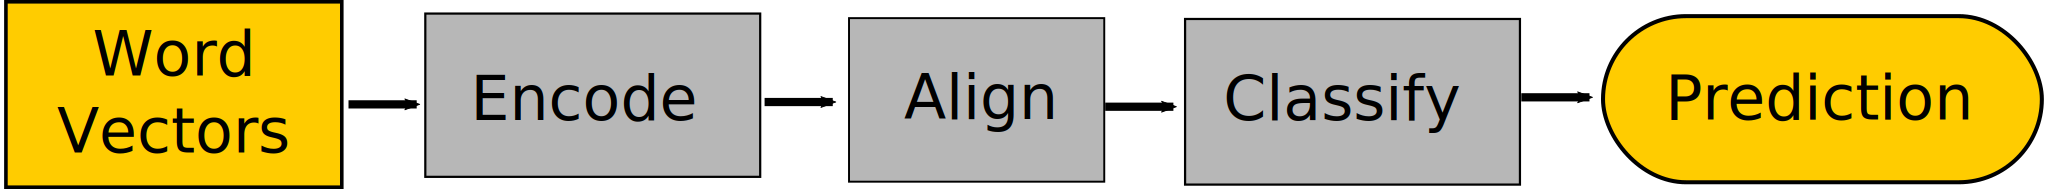
\includegraphics[width=1.0\linewidth]{end2end}
 \caption{End-to-end attention based model.}
\label{fig:modelPipeline}
\end{figure}

\subsection{Neural Network Model in NLP}
%\shusen{neural linguistic models?}
%\shusen{What is the basic understanding of neural network What is the end-to-end}
There are many connection and distinction between neural network model employed for vision tasks and NLP tasks.
On the one hand, as discussed in the introduction, the discrete nature of words and sentences presents additional challenge for
interpreting the NLP model.
%
On the other hand, a majority of recent NLP neural networks share the nature of
end-to-end model, where the entire model operates as a black-box that takes
vectorized input and yields final prediction for a specific task.
Therefore, to make sense of how predictions are made inside of end-to-end neural models, it is important to
explore the interaction between intermediate representations and predictions.

Many of the recent NLP end-to-end neural network models, despite having potentially drastic different network architecture, share a similar high-level design that consist of three distinct stages (encode, attent/align, classify, see Fig.~\ref{fig:modelPipeline}). 
These models usually take pre-trained word vectors (a numerical vector representation of individual words, where the semantic similarities are encode by distances in the high-dimensional space~\cite{MikolovSutskeverChen2013, PenningtonSocherManning2014}) as input, the 

\subsection{Attention Mechanism}
\label{sec:attention}
The introduction of attention mechanism~\cite{bahdanau2014neural} allows
pairwise interaction between hidden states. This interaction can be naturally explained
as a form of alignment which exposes an interpretable layer in end-to-end neural networks.
Recently attention has contributed to many strongly-performed NLP models
~\cite{parikh2016emnlp},~\cite{rush2015neural},~\cite{yang2016hierarchical},
~\cite{seo2016bidirectional},~\cite{schwartz2017high}.
We will focus on its application in Natural Language Inference task as proposed in~\cite{parikh2016emnlp}.
However notice that our visualization can be generalized to other attention models as well.

\begin{figure}[htbp]
\centering
\vspace{-2mm}
 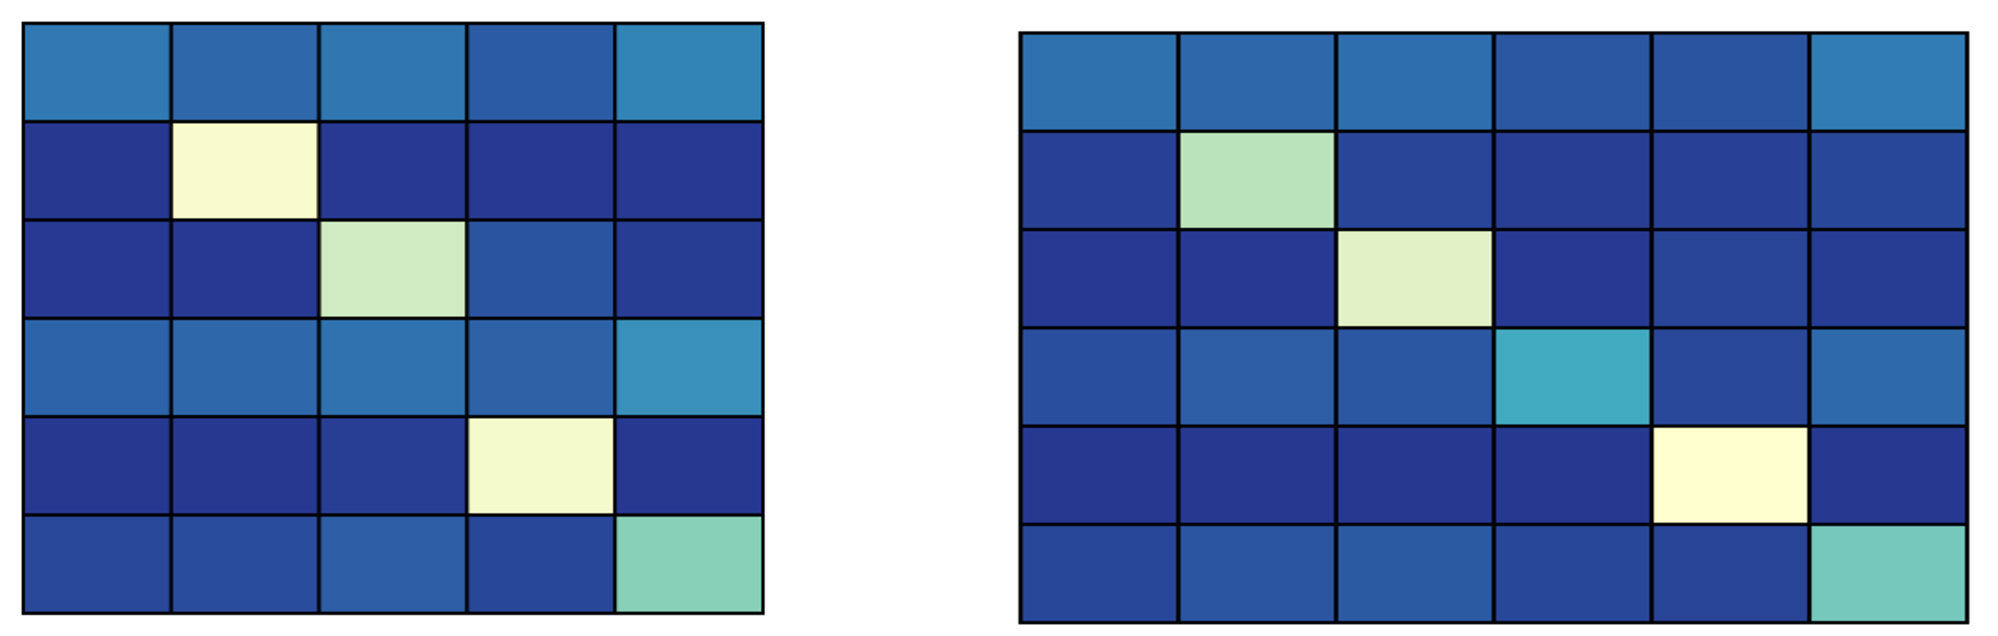
\includegraphics[width=0.9\linewidth]{attentionIllustration}
 \caption{Attention illustrate. The soft alignment between two sentences.}
\label{fig:attention}
\end{figure}

% \begin{itemize}
%     \item what is the textaul entailment problem
%     \item the importance of textual entailment problem
%     \item how easily can the visualization method extends other NLP problem
% \end{itemize}
